\documentclass[10pt,a4paper]{article}
\usepackage[latin1]{inputenc}
\usepackage{amsmath}
\usepackage{amsthm}
\usepackage{amsfonts}
\usepackage{amssymb}
\usepackage{graphicx}
\author{Yuqian Li}
\title{Analysis of Defender System in LiveS Cube}
\date{}

\newtheorem{mydef}{Definition}
\newtheorem{mylemma}{Lemma}
\newtheorem{mytheorem}{Theorem}
\newtheorem{mycor}{Corollary}


\begin{document}
\maketitle
%\paragraph*{Abstract}{
\begin{abstract}
	Some information has a very small input set. For example
	cellphone numbers has only $2^{32}$ possible values. In that case, any
	determinant encryption could only
	achieve a very low entropy bounded by the size of input set.
	Again, for example, the entropy can't exceed $32$ for an input set
	of size $2^{32}$. However, the determinant encryption is required
	in situations such as hashing or generating an index or identity for a
	given information. To ensure the security in a theoretical aspect
	for such cases, conditional entropy is used instead of mere entropy.
	The conditional entropy measures the difficulty for an adversary to
	derive the information considering all related information 
	that adversary has already achieved.
	The defender system is a subsystem in LiveS Cube system
	designed to ensure a relatively high lower
	bound for conditional entropy even with a computationally-unbounded adversary.
	In this paper, a very easy proof is given to show the lower bound.
\end{abstract}
%}

\section{Introduction}
	Determinant encryption for an information from
	a very small input set is important for some social
	network systems such as LiveS Cube. LiveS Cube is a system to
	build a social network based on the address books in cellphones.
	In that social network, each node is indexed by an encrypted information generated
	from the cellphone number
	of its user. Therefore, a huge network could be easily established
	using existing address books in numerous of cellphones without
	any additional effort of the users. However, cellphone numbers are
	one of the most important privacy so the security of preventing
	someone getting the corresponding cellphone number from its index 
	is the base of the system.
	
	But the security
	of such determinant encryption is hard to be guaranteed. For example, an
	adversary might enumerate all possible values from the
	input set and establish a table maps any encrypted
	information to its plain information as long as the encryption
	does not change. In such case, the conditional entropy
	is $0$ since there's no randomness for the adversary with that table.
	Even for a large input set which has a quite high entropy, a
	computationally-unbounded adversary could establish that table
	fast and the conditional entropy drops to $0$, which means that the
	adversary knowns everything. So it's not the mere entropy that
	determines the security, but the conditional entropy.
	
	Therefore, even for the very small input set that has a very low
	higher bound for entropy, there is still possibility to ensure the
	theoretical security by given a lower bound for conditional entropy.
	The defender model is an easy model based on a simple idea to achieve that goal.
	This model is used in LiveS Cube system so a defender system is made.
	The analysis in the following sections is mainly based on that system.
	The result shows that the system could ensure a relatively high lower bound
	in a very efficient way. Since the analysis is quite simple, the
	bound estimated is believed not to be so tight. 
	Considering the result derived by some other
	more complex, however not accurate, only approximate ways, it is believed
	that the tight lower bound for this system is much higher than what we proved.
	
	In the following sections, firstly the defender model and system will be
	introduced. Then a simple proof for the lower bound of conditional entropy
	is given. Finally there's some more discussions about the meaning of
	conditional entropy and other approximate ways to estimate the conditional
	entropy.
	
	Though defender system is currently used for only one specific LiveS Cube System,
	it is believed to be useful for many other social network
	systems for the following reasons. 
	
	Firstly, more and more social network systems
	begin to notice that the security based on well performed administrators and
	unhackable servers is not reliable since human mistakes and 
	server vulnerabilities are unpredictable. Hardly anyone can still totally 
	trust servers and administrators after so many successful attacks every day.
	The security of defender system is theoretically proved based on distributed
	clients and a specific hardware with strictly designed interface. Distributed 
	clients are better than one central server because one mistake in a client would not
	take the whole system and all other clients down[ref to distributed OSN]. 
	However, only having distributed clients is not convenient as client/server
	when clients are not always online[check and ref]. So
	one specific hardware is introduced in server to
	guarantee strictly determinant behaviours instead of unpredictable behaviours
	, so the complex security problems of a server in the unknown network world
	become traditional security problems of protecting the hardware from being damaged in real world. Meanwhile,
	the convenience of client/server mode is preserved.
	
	Secondly, not only password is worth being protected, identity is also worth being protected as
	so many new social networks emerges every day. Some research[ref to personal info leakage] has already shown
	that one human could only remember a small number of passwords so one user often
	uses the same password for many many network systems. Some network systems may be
	so vulnerable, or perhaps that system is just a fishing website to get password, so
	password may be easily gotten by others in some systems. And in many other network
	systems where the user uses the same password which is known to others, 
	once the identity is also known to others,
	the security no longer holds. Even if the password is still unknown, knowing identity
	easily is still a problem: spam emails can be sent if they know your identity in an email system,
	nuisance calls can be made if they know your identity in a mobile system. However,
	to ensure the security of identity is harder than password because the identity should
	be human friendly and very easy to remember not only for the owner, but also for his or her friends.
	That means only determinant encryption can be made for very low entropy information, as 
	same as what LiveS Cube faces.
	
	Till now, identity is not well protected and is always stored as plain text in server's database. That means
	a successful hack or an administrator's mistake could leak all those identities easily.
	
\section{Defender Model and System}
	\subsection{Defender Model}
		Defender model is a very simple model that
		is not based on formal information theory.
		The adversary is called attacker in this model.
		The attacker can launch some attacks and after
		each attack, the attacker gains some useful information.
		Once the attacker gains enough information, the security
		is compromised.
		
		Initially, the attacker knows nothing. After
		each attack, the information attacker gains
		is described as a function $f_A$, so we define:
		\begin{align}
			I_0 &= 0\\
			I_n &= f_A(I_{n-1})\label{AONLY}
		\end{align}
		Here $I_i \in [0, 1]$ describes the amount of information
		to compromise the security after $i$
		rounds of attack: $0$ for nothing, $1$ for enough
		information to compromise the security.
		
		For a simple attacker who enumerates all possibilities, the
		function $f_A$ is quite simple:
		\begin{align}
			I_n = f_A(I_{n-1}) = I_{n-1}+c\label{AONLYE}
		\end{align}
		Here $c$ is a constant depend on how many possibilities the
		attacker has to enumerate. For example, if there are
		$m$ possibilities, $c = 1/m$. In normal situations, $m$ is more
		than $2^{128}$, so such a simple attacker just needs too many rounds
		of attack to compromise the security. Therefore, the system with
		a large $m$ is safe if the attacker is computationally-bounded.
		
		However, in some situations, the $m$ is very small. In such cases,
		we must introduce a defender against that attacker to ensure the
		security. The defender's action is also described as a function $f_D$
		so the equation(\ref{AONLY}) above becomes:
		\begin{align}
			I_n = f_A(f_D(I_{n-1}))
		\end{align}
		
		For simple attacker who enumerate all possibilities,
		there is a simple but effective defender 
		who periodically reduces the information 
		attacker has in a constant rate, so
		the equation(\ref{AONLYE}) becomes
		\begin{align}
			I_n = f_D(I_{n-1})+c = I_{n-1}/d+c
		\end{align}
		Here $d > 1$ is the rate to reduce the information.
		It can be easily conducted that:
		\begin{align*}
			\lim_{n \rightarrow \infty} I_n &= \lim_{n \rightarrow \infty} \sum_{0 \leq i < n} \frac{c}{d^i}\\
				&= \frac{c}{d-1}
		\end{align*}
		
		This means that for a small $d$ such as $2$, even $c$ is as large as
		$0.1$ and the attacker is computationally-unbounded, the attacker
		could never compromise the security.
		
	\subsection{Defender System}\label{sec_ds}
		Inspired by the simple defender model, the defender system is implemented
		in LiveS Cube[ref] system which has to generate an index
		from a given cellphone number. The defender system is to prevent attackers
		from knowing the corresponding cellphone number from its index.
		
		Define the set of cellphone number as $\mathcal X = \{x | \text{$x$ is a cellphone number}\}$.
		There's a function $f: \mathcal X \rightarrow F$ to generate index $h = f(x) \in F$ for
		a given $x$. As described before, the cellphone number set $\mathcal X$ has a very small
		size about $2^{32} \approx 10^{11}$. For a given index $h^*$, a simple attacker
		can enumerate all possible $x$ to see whether $f(x) = h^*$. Therefore, in defender
		model:
		\begin{align*}
			f_A(I_{n-1}) = I_{n-1}+c = I_{n-1}+2^{-32}
		\end{align*}
		
		So the security will be compromised after $2^{32}$ rounds of attack if there's
		no defender. The defender system is going to fullfil the defender
		function $f_D(I_{n-1}) = I_{n-1}/2$ by generating new indexes.
		In LiveS Cube system, the indexes and corresponding data entries are stored
		in database which we think attacker may have an access to. To generate
		new indexes, the system has to send indexes and data entries to a 
		secured module
		and get new indexes and data entries from that module. If attacker
		could track each new index and its old index, there's no loss of information 
		for attacker. Therefore, we have to make sure that the attacker couldn't track
		the procedure to update the indexes.
		To do that, the module is implemented in a special hardware that nobody
		could see what's going on inside the hardware without damaging it in real world.
		The best strategy againt the attacker 
		is to send all indexes and data entries to that hardware and then
		retrieve all new indexes and data entries together. By doing that, the attacker
		loses all information, which means $f_D(I_{n-1}) = 0$. However, the entries
		in database may be too many for that hardware to store. Therefore, the system
		sends two indexes and data entries from the database to hardware in one time and
		then retrieve their new indexes and data entries. After that, the attacker can
		only guess which new index is from which old index and there are $2$ possibilites.
		Thus, the defender system fullfils the equation $f_D(I_{n-1}) = I_{n-1}/2$.
		
		In short, in defender system,
		there's a function $g: F \rightarrow F$ regenerating 
		new indexes from old indexes. The defender system
		will randomly choose $h_1, h_2 \in F$ that have
		not been regenerated yet in each time and generate
		$h_1', h_2' \in F$ in a way that attacker can't tell whether
		$h_1' = g(h_1), h_2' = g(h_2)$ or $h_2' = g(h_1), h_1' = g(h_2)$.
		By doing that, the information like $f(x) = h$ becomes
		information that there's $1/2$ chance $f'(x) = h_1'$ and $1/2$ chance $f'(x) = h_2'$.
		Thus $f_D(I_{n-1}) = I_{n-1}/2$ is achieved.
		
		In real system, doing such a defend operation to update whole
		database after each possible attack costs too much.
		Therefore, the defend operation is required after $m$
		possible attack operations rather than one. Under this
		new condition, $f_D$ is unchanged, while $f_A(I_{n-1}) = I_{n-1}+c$
		becomes $f_A(I_{n-1}) = I_{n-1}+c' = I_{n-1}+m \cdot c$.
		The $m$ can be tuned in balance of security and the
		efficiency of system.
		
		The conclusions about the defender model
		and system above are not strictly
		proved because defender model itself
		is not well defined in theoretical aspect. 
		However this is a comprehensive explanation to show how and why
		defender system works. In the following section, a mathematical proof
		will be given based on information theory to demonstrate that
		the defender system can truly ensure the security even for
		a computationally-unbounded attacker, consistent with what
		is claimed here.
		
\section{Analysis of Conditional Entropy}
	\subsection{Definition and Examples}
		In this subsection, a brief definition for entropy and conditional
		entropy is given. Besides, the formal definition of defender system
		and its behaviour is given.
		Some additional examples are taken to further
		demonstrate the relation between conditional entropy and
		the security. Feel free to skip the content about
		the definition of entropy and conditional entropy if you are familiar
		with them.		
		
		\begin{mydef}[Entropy]
			The entropy of a discrete random variable $X$ with
			possible values $\{x_1, x_2, \ldots, x_n\}$ is
			\begin{align}
				H(X) = -\sum_{i=1}^n p(x_i)\log p(x_i)
			\end{align}
			where $\log$ refers to $\log_2$ in our context.
		\end{mydef}
		
		Correspondingly, in defender system, define
		\begin{mydef}\label{def2}
			$\mathcal{X} = \{x_1, x_2, \ldots, x_n\}$ is the set of all possible 
			primary images\footnote{the primary images are cellphone numbers
			in LiveS Cube system} that index $h_i = f(x_i)$ can be calculated.
			Suppose $h^*$ is the index that attacker wants to
			get its primary image $x^* \in \mathcal{X}$ satisfying $f(x^*) = h^*$.
			The discrete random variable $X$ is the
			primary image guessed by the attacker. For convenience,
			suppose $n = 2^D$.
		\end{mydef}
		
		In ideal situation, the attacker has no related information, so $X$ should
		be uniformly distributed. In such case, the entropy is simply:
		\begin{align*}
			H(X) &= -\sum_{i=1}^{2^D} 2^{-D} \log 2^{-D}\\
				&= D
		\end{align*}
		
		\begin{mydef}[Conditional Entropy]
			For a discrete random variable $X$ with
			possible values set $\mathcal X$,
			suppose that there is another random
			variable $Y$ with possible values
			set $\mathcal{Y}$, the conditional entropy
			of $X$ given $Y$ is
			\begin{align}
				H(X|Y) &= \sum_{y \in \mathcal Y} p(y) H(X | Y = y)\\
					&= -\sum_{y \in \mathcal Y} p(y) \sum_{x \in \mathcal X} p(x|y) \log p(x|y)\\
					&= -\sum_{y \in \mathcal Y} \sum_{x \in \mathcal X} p(x, y) \log p(x|y)
			\end{align}
		\end{mydef}
		
		In our context, random variable $Y$ represents the related information
		that attacker has. For example, when attacker has enumerated only one
		$x$ to calculate $f(x)$, $Y$ can be defined as $Y^{(1)}$:
		\begin{align*}
			&\mathcal Y^{(1)} = \{y \: | \: \exists x \in \mathcal X, f(x) = y\}\\
			&\forall y \in \mathcal Y^{(1)}, \; p(Y^{(1)} = y) = \frac{1}{n} = \frac{1}{2^D}\\
			&p(x|y) = \begin{cases}
				\frac{1}{n-1}, &y \neq h^*\\
				0, &y = h^* \text{ and } f(x) \neq y\\
				1, &y = h^* \text{ and } f(x) = y
			\end{cases}
		\end{align*}
		
		Similarly, when attacker has enumerated $m$ different primary images, $Y$ can be defined
		as:
		\begin{equation*}
			\mathcal Y^{(m)} = \{ y = \{y_1, y_2, \ldots, y_m\} \: | \: \exists x_i \in \mathcal X, f(x_i) = y_i\}
		\end{equation*}
		\begin{equation*}
			\forall y \in \mathcal Y^{(m)}, \; p(Y^{(m)} = y) = \frac{1}{\binom{n}{m}}
		\end{equation*}
		\begin{equation*}
			p(x|y) = \begin{cases}
				\frac{1}{n-m}, &h^* \notin y\\
				0, &h^* \in y \text{ and } f(x) \neq h^*\\
				1, &h^* \in y \text{ and } f(x) = h^*
			\end{cases}
		\end{equation*}
		
		Therefore, $H(X | Y^{(m)})$ can be calculated as:
		\begin{align*}
			H(X | Y^{(m)}) &= \sum_{y \in \mathcal Y^{(m)}} p(y) H(x | Y^{(m)} = y)\\
				&= \sum_{h^* \in y} p(y) H(x | Y^{(m)} = y) + \sum_{h^* \notin y} p(y) H(x | Y^{(m)} = y)\\
				&= 0+\frac{\binom{n-1}{m}}{\binom{n}{m}} \log(n-m)\\
				&= \frac{n-m}{n} \log(n-m)
		\end{align*}
		
		It's clear that as $m$ increases, 
		the conditional entropy decreases and drops to $0$ when $m = n-1$. 
		Consistent with the intuition, the conditional
		entropy which notifies the security decreases about linearly when $m$ is small 
		compared with $n$.
		
	\subsection{Proof of a Simple Lower Bound}
		As the example above demonstrates, the key to the calculation
		of conditional entropy $H(X|Y)$ is the definition of the condition $Y$.
		To make a simple proof for the lower bound, we can simplify the
		condition to achieve that. Before defining $Y$, let's
		more clearly clarify how defender system behaviours first. Clear
		definition of $X$ can be found in definition \ref{def2}
		if that is unclear.
		
		The defender system will allow attacker to do at most $m$ possible
		attack operations before one defend operation. More specifically, between
		two operations of updating the whole database about the indexes and data entries,
		at most $m$ indexes are calculated from primary indexes. It's formally defined
		as:
		\begin{mydef}[Defender System]
			There are functions $f_0, f_1, f_2, \ldots$ where
			$f_0$ denotes the most recent function $f: \mathcal{X} \rightarrow F$
			to generate an index $f(x) = h \in F$ from primary image $x$. 
			Besides, $f_1$ denotes the last one used before update, $f_2$ for the last but one and so on.
			There are also functions $g_0, g_1, g_2, \ldots$ where
			$g_i$ is an update function $g_i: F \rightarrow F$ such that
			$f_i(x) = g_i(f_{i+1}(x))$. Considering the capability of hardware and security,
			$g_i$ is designed in a way that:
			\begin{align*}
				\{g_i(f_{i+1}(x_1)), g_i(f_{i+1}(x_2))\} = \{ f_i(x_1), f_i(x_2)\} = G_i(x_1, x_2)
			\end{align*}
			But attacker don't know whether $g_i(f_{i+1}(x_1)) = f_i(x_1)$ or
			$g_i(f_{i+1}(x_1)) = x_2$. 
			Here, set $G_i$ is defined for convenience in later proof and
			it's also totally random
			to the attacker. \footnote{See section \ref{sec_ds} for the purpose
			of $g$}
		\end{mydef}
		
		To better describe the interaction between attacker and defender
		system, candidate sets and collision sets is defined as following
		\begin{mydef}[Candidate and Collision Set]
			Candidate sets are $C_0, C_1, C_2, \ldots$ recursively defined as
			\begin{align*}
				C_0 &= \{h^*\}\\
				C_i &= \{h | \exists G_{i-1}(x_1, x_2),
					g_{i-1}(h) \in G_{i-1}(x_1, x_2) \text{ and } 
					G_{i-1}(x_1, x_2) \cap C_{i-1} \neq \emptyset \} (i \geq 1)
			\end{align*}
			Here $h^*$ is the index that attacker wants to know its primary image
			$x$ such that $f_0(x) = h^*$. And collision sets are $K_0, K_1, K_2, \ldots$ where
			\begin{align*}
				K_i = \{h | f_i(x) = h \text{ is enumerated by attacker and } h \in C_i \}
			\end{align*}
		\end{mydef}
		
		The candidate set $C_i$ can be described as the set of indexes of $f_i$ that could be
		updated to $h^*$ through $g_0, g_1, \ldots, g_{i-1}$. The collision set $K_i$ is the
		subset of $C_i$ that are enumerated by the attacker. Since $g_i$ and $f_i$ is random
		to attacker and a maximum of $m$ indexes are allowed to be calculated using $f_i$, 
		the random distribution of $|K_i|$ is only related to $|C_i|$ and has a maximum
		of $m$. 
		
		Now condition $Y$ will be simply defined as following:
		\begin{mydef}[Simple Condition $Y_d$]
			$Y_d$ is a random variable with values set
			$\mathcal Y = \{ \alpha, \beta \}$ where
			$Y_d = \alpha$ means that $|C_d| = 2^d$
			and $|K_0| = |K_1| = \ldots = |K_{d-1}| = 0$.
			Otherwise $Y_d = \beta$.
		\end{mydef}
		
		By the definition of conditional entropy,
		\begin{align*}
			H(X|Y) &= p(Y = \alpha) H(X | Y = \alpha) + p(Y = \beta) H(X | Y = \beta)\\
				&\geq p(Y = \alpha) H(X | Y = \alpha) + 0
		\end{align*}
		
		To prove a simple lower bound, three lemmas are proposed.
		The first one shows a lower bound for $H(X | Y = \alpha)$
		and the other two prove a lower bound for $p(Y = \alpha)$.
		The final lower bound of $H(X | Y)$ will be achieved by putting
		them together.
		
		\begin{mylemma}\label{lem1}\footnote{See definition\ref{def2} for $D$}
			$H(X|Y_d = \alpha) \geq d \cdot (1-\frac{m^2}{2^D-dm+1})$
		\end{mylemma}
		
		\begin{proof}
			When $Y_d = \alpha$, the attacker
			is just unlucky in last $d$ updates
			and our defender system is lucky
			to expand $C_d$ quickly.
			In this case, the best that attacker
			may have is to know all relations
			like $f_d(x) = h$ for $x \in \mathcal X$.
			
			In addition, $H(A) \geq H(A|B)$ for
			any $A, B$, which simply means that knowing something
			more can never be a bad thing. Let $A = X | Y_d = \alpha$
			and $B$ be whether there is any $x \in C_d$ that
			has been enumerated using $f_0, f_1, \ldots, f_{d-1}$ 
			by the attacker or not.
			Then
			\begin{align*}
				H(X | Y_d = \alpha) &= H(A)\\
					&\geq H(A | B)\\
					&\geq p(B = false) \cdot H(A | B = false)
			\end{align*}
			
			When $B = false$, each $f_d(x_i) = h_i \in C_d$
			has an equal chance of $f_0(x_i) = h^*$. Therefore
			we have:
			\begin{align*}
				H(A | B = false) &\geq -\sum_{i = 1}^{2^d} \frac{1}{2^d} \log(\frac{1}{2^d})\\
					&= d
			\end{align*}
			
			For $p(B = false)$, use simple counting method:
			\begin{align*}
				p(B = false) &= \frac{\binom{n-dm}{m}}{\binom{n}{m}}\\
					&= \frac{(n-m)(n-m-1)\ldots(n-dm-m+1)}{n(n-1)\ldots(n-dm+1)}\\
					&\geq (\frac{n-dm-m+1}{n-dm+1})^m\\
					&= (1-\frac{m}{n-dm+1})^m\\
					&\geq 1-\frac{m^2}{n-dm+1}
			\end{align*}
			
			So finally:
			\begin{align*}
				H(X | Y_d = \alpha) &\geq p(B = false) \cdot H(A | B = false)\\
					&\geq d \cdot (1-\frac{m^2}{n-dm+1})\\
					&= d \cdot (1-\frac{m^2}{2^D-dm+1})
			\end{align*}
		\end{proof}
		
		To prove a lower bound of $p(Y = \alpha)$, the following fact is used.
		$(Y = \alpha)$ is equivalent to $\left(|C_d| = 2^d \text{ and } |K_i| = 0	\; (0 \leq i < d)\right)$.
		Therefore 
		\begin{align*}
			p(Y = \alpha) = p(|C_d| = 2^d) \cdot p(|K_i| = 0	\; (0 \leq i < d) \; \backslash \; |C_d| = 2^d)
		\end{align*}
		The following two lemmas are for $p(|C_d| = 2^d)$ and $p(|K_i| = 0	\; (0 \leq i < d) \; \backslash \; |C_d| = 2^d)$ 
		respectively.
		
		\begin{mylemma}
			\begin{align*}
				p(|C_d| = 2^d) \geq 1-\frac{d \cdot 2^{2d-2}+d \cdot 2^{d-1}}{2^D-1}
			\end{align*}
		\end{mylemma}
		
		\begin{proof}
			$|C_d| = 2^d$ means that $G_i(x_1, x_2) \cap C_i \leq 1$
			for all $G_i(i \leq d-1)$. So
			\begin{align*}
				p(|C_d| = 2^d) &= \prod_{i=0}^{d-1} p\left((\forall G_i(x_1, x_2), G_i(x_1, x_2) \cap C_i \leq 1)
					 \; \backslash \; |C_i| = 2^i\right)
			\end{align*}
			
			It's obvious that
			\begin{align*}
			&p\left((\forall G_i(x_1, x_2), G_i(x_1, x_2) \cap C_i \leq 1) \; \backslash \; |C_i| = 2^i\right)\\
			&\geq \\
			&p\left((\forall G_{d-1}(x_1, x_2), G_{d-1}(x_1, x_2) \cap C_{d-1} \leq 1) \; \backslash \; 
				|C_{d-1}| = 2^{d-1}\right)
			\end{align*}
			
			Therefore
			\begin{align*}
				&p(|C_d| = 2^d) \\
				&\geq p\left((\forall G_{d-1}(x_1, x_2), G_{d-1}(x_1, x_2) 
					\cap C_{d-1} \leq 1) \; \backslash \; |C_{d-1}| = 2^{d-1})\right)^d\\
				&= P^d
			\end{align*}
			
			$P$ here can be easily estimated by counting method as
			\begin{align*}
				P &= \frac{(n-2^{d-1})(n-2^{d-1}-1)\ldots(n-2^d+1)\cdot (n-2^d-1)!!}{(n-1)!!}\\
					&= \frac{(n-2^{d-1})(n-2^{d-1}-1)\ldots (n-2^d+1)}{(n-1)(n-3)\ldots(n-2^d+1)}
			\end{align*}
			
			Since
			\begin{align*}
				\frac{n-2^{d-1}-i}{n-1-2i} \geq \frac{n-2^{d-1}-j}{n-1-2j} & \text{ when } i \geq j
			\end{align*}
			
			It can be conducted that
			\begin{align*}
				P &= \frac{(n-2^{d-1})(n-2^{d-1}-1)\ldots (n-2^d+1)}{(n-1)(n-3)\ldots(n-2^d+1)}\\
					&\geq (\frac{n-2^{d-1}}{n-1})^{2^{d-1}}
			\end{align*}
			
			Thus
			\begin{align*}
			p(|C_d| = 2^d) &\geq P^d\\
				&\geq (\frac{n-2^{d-1}}{n-1})^{d \cdot 2^{d-1}}\\
				&= (1-\frac{2^{d-1}+1}{n-1})^{d \cdot 2^{d-1}}\\
				&\geq 1-\frac{d \cdot 2^{2d-2}+d \cdot 2^{d-1}}{n-1}\\
				&= 1-\frac{d \cdot 2^{2d-2}+d \cdot 2^{d-1}}{2^D-1}
			\end{align*}
		\end{proof}
		
		\begin{mylemma}
			$p(|K_i| = 0	\; (0 \leq i < d) \; \backslash \; |C_d| = 2^d) 
				\geq 1-\frac{m^2}{2^D-2^{d-1}+1}$
		\end{mylemma}
		
		\begin{proof}
			\begin{align*}
				&p(|K_i| = 0	\; (0 \leq i < d) \; \backslash \; |C_d| = 2^d) \\\
					&\geq p(|K_{d-1}| = 0 \; \backslash \; |C_{d-1}| = 2^{d-1})^d\\
					&= \left(\frac{\binom{n-2^{d-1}}{m}}{\binom{n}{m}} \right)^d\\
					&\geq 1-\frac{m^2}{n-2^{d-1}+1}	\; \text{ (see proof of lemma\ref{lem1} for similar conclusion})\\
					&= 1-\frac{m^2}{2^D-2^{d-1}+1}
			\end{align*}
		\end{proof}
		
		By putting them together, here comes the lower bound
		\begin{align*}
			H(X | Y_d) &\geq p(Y_d = \alpha) \cdot H(X | Y_d = \alpha)\\
				&= p(|C_d| = 2^d) \cdot p(|K_i| = 0	\; (0 \leq i < d) \; \backslash \; |C_d| = 2^d) \cdot H(X | Y_d = \alpha)\\
				&\geq (1-\frac{d \cdot 2^{2d-2}+d \cdot 2^{d-1}}{2^D-1})
					\cdot (1-\frac{m^2}{2^D-2^{d-1}+1}) 
					\cdot (1-\frac{m^2}{2^D-dm+1}) \cdot d 
		\end{align*}
		
		Note that the condition $Y_d$ here contains all the
		information that attacker can have. It assumes that
		the attacker is computationally-unbounded and he has
		been using the system to enumerate (primary image, index) pairs
		for an infinite long time. Also note that the formula
		satisfies arbitrary number $d$. Thus, the lower bound
		of $H(X | Y)$ is the maximum value of that formula
		over all possible $d$.
		As a result, this is our final theorem:
		\begin{mytheorem}\label{thm1}
			In defender system, one index's corresponding
			primary image's conditional entropy has a lower bound of
			\begin{align*}
				\max_{0 \leq d \leq D} \left\{ (1-\frac{d \cdot 2^{2d-2}+d \cdot 2^{d-1}}{2^D-1})
					\cdot (1-\frac{m^2}{2^D-2^{d-1}+1}) 
					\cdot (1-\frac{m^2}{2^D-dm+1}) \cdot d \right\}
			\end{align*}
			considering all the information
			that a computationally-unbounded attacker can
			have in an infinite long time. Here $m$ is
			the maximum number of indexes that are allowed to be calculated
			between defend operations and $D = \log(n)$ denotes the
			logarithm of the size of primary image set.
		\end{mytheorem}
		
	\subsection{Concrete Lower Bound and Approximate Estimation}
		In LiveS Cube system, $D = 32$ and $m$ should be
		choosed in balance of security and efficiency.
		
		In the following graph, the simple lower
		bound we proved when $m = 2^{12}, 2^{13}, 2^{14}, 2^{15}$ is given:
		
		\begin{center}
		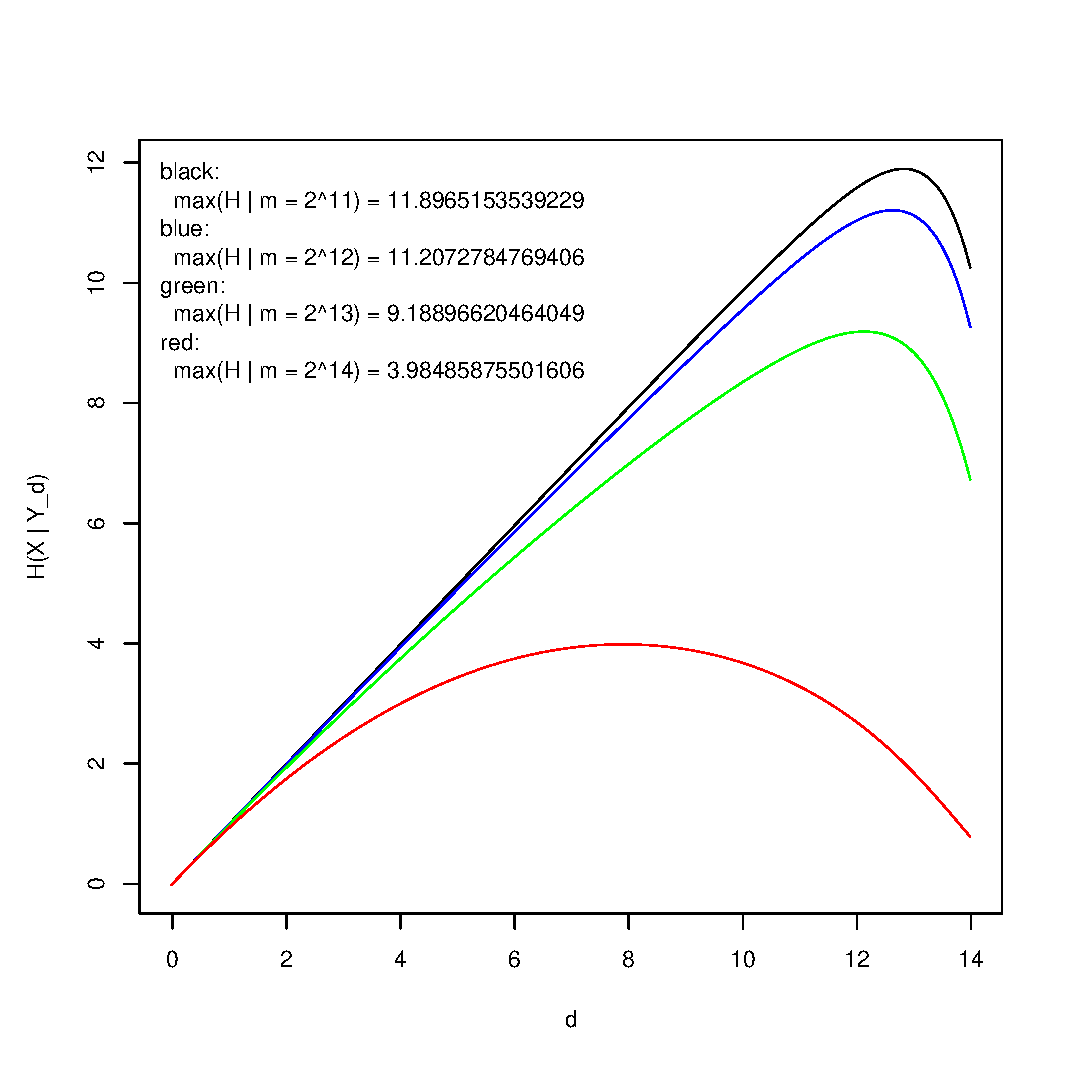
\includegraphics[scale=0.6]{lb_m.eps}
		\end{center}
		
		Since our lower bound in theorem\ref{thm1} is a maximum value
		over $d$, the $x$-axis is $d$ and the peak of each line
		is the lower bound for each $m$. As it shows, when $m = 2^{14} = 16384$, the lower
		bound is about $10.84$. This means that the system can achieve
		a relative high lower bound and keep its efficiency at the same time:
		there is only one update operation after tens of thousands of index calculations.
		
		By observing the formula
		of theorem\ref{thm1}, it's clear that $d \approx D/2$ is a
		breakpoint. Before that point, the lower bound holds and
		decreases slowly. This is very consistent with this
		specific situation that $D = 32$.
		
		In fact, the proved lower bound in theorem\ref{thm1} is so
		simple and the tight lower bound is expected to be much higher.
		Orbserving the proof of theorem\ref{thm1}, only the
		entropy in the situation $Y = \alpha$ is count and
		all other entropy is considered to be $0$. However, in
		many situations that $Y = \beta$, there is still a high entropy.
		What's more, $B = false$ is also assumed and the attacker is
		given an extra information about whether all his enumerated $x$
		in recent $d$ updates are in candidate set $C_d$ or not, though
		in real situation this is unknown to the attacker.
		
		However, to have a strictly proved and tight lower bound
		is a little hard.
		So there's an approximate lower bound which is not
		strictly proved, but should be more tight.
		In this approching,
		the size of candidate set is
		considered to be growing in an equivalent
		constant rate $r \in (1, 2)$ which
		should be very close to $2$.
		And in collision set $K_i$, each
		element has an equal chance of
		$r^{-i}$ to become $h^*$.
		Suppose that the attacker
		has enumerated $f_i(x) = h$
		for $k$ rounds, i.e. $0 \leq i < k \leq \log_r(n)$. Here
		$i < \log_r(n)$ because when
		$|C_i| = n$, the information that
		attacker can still acquire through
		enumeration is considered to be $0$.
		Under these unproved assumptions,
		a formal proof can be given to show that the lower bound
		$H(X | Y) \geq 18$ holds when $m = 2^{20}$. 
		The detailed derivation is however too complex
		to write here.
		
	\subsection{Experimental Evaluation}
		In our simple proof of the lower bound, $p(|C_d| = 2^d)$,
		$p(|K_i| = 0 \; (i \leq 0 < d) \; \backslash |C_d| = 2^d)$ and $p(B = false)$ are 
		three key points to the final result.
		They represent that candidate sets are maximized in
		last $d$ updates, collision sets are minimized in
		last $d$ updates and candidate set $C_d$ is totally unknown
		to the attacker respectively.
		Lower bound for each of them has been proved:
		\begin{align*}
			p(B = false) &\geq 1-\frac{m^2}{2^D-dm+1}\\
			p(|C_d| = 2^d) &\geq 1-\frac{d \cdot 2^{2d-2}+d \cdot 2^{d-1}}{2^D-1}\\
			p(|K_i| = 0 \; (i \leq 0 < d) \; \backslash |C_d| = 2^d) &\geq 1-\frac{m^2}{2^D-2^{d-1}+1}
		\end{align*}
		
		By putting them together, lower bound $H(X | Y_d)$ is achieved:
		\begin{align*}
			H(X | Y_d) &\geq p(B = false) \cdot p(|C_d| = 2^d) \cdot 
				p(|K_i| = 0 \; (i \leq 0 < d) \; \backslash |C_d| = 2^d) \cdot d\\
				&\geq (1-\frac{d \cdot 2^{2d-2}+d \cdot 2^{d-1}}{2^D-1})
					\cdot (1-\frac{m^2}{2^D-2^{d-1}+1}) 
					\cdot (1-\frac{m^2}{2^D-dm+1}) \cdot d 
		\end{align*}
		
		For convenience, write $p(|C_d| = 2^d)$,
		$p(|K_i| = 0 \; (i \leq 0 < d) \; \backslash |C_d| = 2^d)$ and $p(B = false)$
		as $p_1, p_2, p_3$ respectively. 
		$p_1 \cdot p_2 \cdot p_3$ can be measured in a real program which 
		simulates the same behaviour as we defined in defender system.
		The proof above can be checked by this experimental measurement.
		Moreover, this experiment will show how tight our lower bound is
		when $H(X | Y_d = \beta)$ and $H(A | B = true)$ is ignored.

\section{Conclusion}
	A simple defender model is proposed to ensure
	the security of low entropy information
	such as cellphone numbers. Based on that, defender system
	 is implemented in LiveS Cube
	system. To have a better and strict analysis, a simple lower bound of conditional
	entropy is proved to show that the security
	is indeed guaranteed in information theory.
	It's also proved that the system can guarantee
	a relative high lower bound and at the same time
	keep a high efficiency.
	
	What conditional entropy really means to
	real situation and what important and practical
	result can we derive from the lower bound of
	conditional entropy is worth researching later.
	It's also good to establish a tighter lower bound
	for the system in the future, although this is
	a little hard.
		
\end{document}
